\input{../Projektarbeit_Bauteileautomat_WIP_begin}

\definecolor{hellblau}{rgb}{0.8,0.8,1}
\definecolor {hellgrün}{rgb}{0.5,1,0.8}
%\usepackage{wrapfig}

\section{Mechanik}


Dieses Kapitel dokumentiert die mechanische Funktionsweise und die Berechnung der zugehörigen Komponenten. Der Automat soll ca. 1000 Boxen enthalten, um eine große Auswahl zu gewährleisten. Damit dies in einer kompakten Bauweise möglich ist, werden drei unterschiedlich große Boxen verwendet. Die Boxen befinden sich in verschiedenen Schächten. 
Ein Schacht besteht aus jeweils zwei L-Profilen, die mit Schrauben an den Aluminiumprofilen der Rückwand befestigt werden. Die Größe der Schächte ist jederzeit änderbar und somit für jede Boxengröße variabel einstellbar. Ein Greifer, der auf X-Y-Z-Achsen verschiebar ist, fährt den ausgewählten Schacht an und greift anschließend die entsprechende Box. An der Seite des Automaten ist ein Rutsche angebracht, die zur Ausgabe der Teile dient. Der Greifer fährt diese an und kann durch ein Drehgelenk die Box um $180^\circ$ drehen und das gewünschte Teil auswerfen.


\subsection{Greifer}

\subsubsection{Anforderungen}


Der Greifer hat den sicheren Transport der Boxen zwischen den Schächten und der Rutsche zu gewährleisten. Er muss ein Drehgelenk beinhalten, das sich um $180^\circ$ drehen lässt. Weiter sind vom Greifer zwei verschieden große Boxen mit einem maximalen Gewicht von 1000g zu befördern. Damit die Ausgabe der Teile nicht zu lange dauert, muss die Geschwindigkeit des Greifvorgangs entsprechend hoch sein.


\subsubsection{Realisierung des Greifers}

Der Greifmechanismus erfolgt über zwei 20cm lange Greifarme aus Aluminium, wobei ein Greifarm fest verbaut ist und der andere über eine Trapezgewindespindel verfahrbar ist. Für den Antrieb der Spindel werden zwei Zahnräder verwendet, welche mit einem Schrittmotor verbunden sind. Damit der bewegliche Greifarm nicht verkantet, wird er über eine zusätzliche Welle geführt. Moosgummi auf dem Greifarm erhöht die Haftkraft zwischen den Boxen und den Greifarmen. Der Drehmechanismus erfolgt ebenfalls über zwei Zahnräder und einen Schrittmotor. Ein Zahnrad ist auf einer Welle befestigt, die auf einer Seite fest mit dem Greifer verbunden ist und auf der anderen Seite in einem Rillenkugellager gelagert ist. Durch das zweite Zahnrad, das durch einen Schrittmotor angetrieben ist, kann die Welle  mit dem Greifer rotiert werden. 


\subsubsection{Antrieb}

Alle relevanten Eigenschaften(Presskraft, Verfahrensgeschwindigkeit und Schrittlänge) sind abhängig vom Schrittmotor 
des Greifmechanismus. Für die richtige Dimensionierung des Schrittmotors sind entsprechende Berechnungen erforderlich.

\begin{itemize}

\item Haltekraft des Greifarms

Das Drehmoment des Motors muss den sicheren Transport einer Box mit einem Gewicht von 1000g gewährleisten. Zur Berechnung des Drehmoments wird die Presskraft benötigt, die der dynamische Greifarm auf die Box ausübt. Hier handelt es sich um einen Erfahrungswert, da verschiedene Berechnungsvariablen (z.b. Reibunkskoeffizent von Polystrol und Moosgummi) nicht vorhanden sind. Der Wert wurde daher auf $F=50N$ ausgelegt und bewußt höher gewählt, damit die Boxen auch bei kleinen Stößen und Vibrationen nicht aus dem Greifarmen rutschen können.\\
\newline

Durch die Umwandlung von einer Drehbewegung in eine Längsbewegung entsteht ein Wirkungsgrad, welcher durch den 
Steigungswinkel des Trapezgewindes und den Gewindereibungswinkel berechnet werden kann.\\

Den Steigungswinkel erhält man durch:

\[tan(\alpha)=\dfrac{P}{d\cdot \pi}=\dfrac{20mm}{4mm\cdot \pi}=\dfrac{5}{\pi}\]

\begin{tabbing}
mit \= P: Spindelsteigung\\
    \> d: Spindelnenndurchmesser  \\
		\> $\alpha$: Steigungswinkel\\
\end{tabbing}

Für ISO-Trapezgewinde mit geschmierter Mutter und einem Reibwert von $\mu=0.04$ erhält man den Gewindereibungswinkel mit:

\[ \rho=\mu\cdot 1.07= 0.04\cdot 1.07=0.043 \]

\begin{tabbing}
mit \= $\rho$: Gewindereibungswinkel\\
    \> $\mu$: Reibwert  \\
\end{tabbing}

Mit dem Steigungswinkel und dem Gewindereibungswinkel kann nun der Wirkungsgrad berechnet werden:

\[\eta=\dfrac{tan(\alpha)}{tan(\alpha +\rho)}=\dfrac{tan(\dfrac{5}{\pi})}{tan(\dfrac{5}{\pi}+0.043)}=3.08\]

\begin{tabbing}
mit \= $\eta$: Wirkunsgrad \\
\end{tabbing}

Das Antriebsdrehmoment der Spindel ergibt sich aus der Presskraft, der Steigung und dem Wirkungsgrad des Trapezgewindes: \\

\[M=\frac{F\cdot P}{1000\cdot 2\pi \cdot \eta}=\frac{50N\cdot 4mm}{1000\cdot 2\pi \cdot 3.08}=0.01Nm\]
\newline

\begin{tabbing}
mit \= M: Antriebsmoment\\
    \> F: Presskraft \\
\end{tabbing}


Auf das Ergebnis müssen die Verluste durch die Lagerung und der Wirkungsgrad der Übersetzung aufgeschlagen werden. Zur Berücksichtigung  dieser Verluste sollte die ausgewählte Leistung des Antriebs um 60\% bis 100\% über dem errechneten Wert liegen.\\

Mit dem Übersetzungsverhältnis der Zahnräder und den Verlusten des Greifmechanismus erhält man das geforderte Drehmoment des Motors durch:

Übersetzungsverhältnis der Zähnrräder:\\
\[i=\frac{z_2}{z_1}=\frac{30}{60}=0.5\]	

das Antriebsmoment des Schrittmotors:\\		
		
\[M_{Motor}=M_{Spindel}\cdot i \cdot R=0.01Nm \cdot 0.5 \cdot 1.6= 8Nmm \]

\begin{tabbing}
mit \= i: Übersetzungsverhältnis\\
    \> R: Reibungsverluste \\
\end{tabbing}






\item Schrittlänge

Die Schrittlänge ist der kleinstmögliche Weg, den der Greifarm zurücklegen kann. Bei einem Schritt des Motors wird dieser Weg zurückgelegt. Alle anderen Wege ergeben sich als ein vielfaches der Schrittlänge. Das weiche Moosgummi auf den Greifarmen und die Elastizität der Boxen erfordern eine feine Abstimmung der Presskraft der Greifarme. Für eine anwendungsgerechte Einstellung ist eine kleine Schrittlänge erforderlich.
\newpage



Mit dem Übersetzungsverhältnis kann die Schrittlänge des Greifers berechnet werden:
\[S=\frac{P}{\frac{360^\circ}{\alpha}}\cdot i=\frac{4mm}{\frac{360^\circ}{1.8^\circ}}\cdot 0.5=0.01mm\]


\begin{tabbing}
mit \= $\alpha$: Schrittwinkel des Elektromotors\\
    \> P: Steigung der Trapezgewindespindel
\end{tabbing}

Die geringe Schrittlänge ist ausreichend um die benötigte Presskraft einzustellen. Toleranzen des Gewindes oder der Schritte des Schrittmotors können vernachlässigt werden.
\newline

 
\item Geschwindigkeit des Greifarms\\

Um einen Schacht anzufahren müssen die Greifarme schon in der richtigen Schachtgröße positioniert werden. 
Die Positionierung findet während der Anfahrt an die jeweiligen Schächte statt. Somit muss nur noch das tatsächliche Greifen in einem gesonderten Arbeitsgang stattfinden. Hier ist der Verfahrensweg so klein $s<5mm$, dass die Geschwindigkeit größtenteils irrelevant ist. 

\end{itemize}



\subsubsection{Kugellager}

Um das Kugellager richtig zu wählen und eine lange Lebensdauer zu garantieren, wird die nominelle Lebensdauer nach 
ISO 281 berechnet:\\

\[L_{10h}=(\frac{C}{P})^p=(\frac{627N}{10N})^3 = 246492\]	


\begin{tabbing}
mit \= p: Lebensdauerexponent (bei Kugellager p=3)\\
    \> C: Dynamische Tragzahl in Kn(aus Lagertabelle des Herstellers) \\
    \> P: Dynamische äquivalente Belastung\\
		\> $L_{10}$: Lebensdauer in Millionen Umdrehungen bei 10\% Ausfallwahrscheinlichkeit
\end{tabbing}


Die nominelle Lebensdauer gibt an, wieviele Umdrehungen $90\%$ der Lager erreichen oder überschreiten bis die ersten Anzeichen von Werkstoffermüdung auftreten. Mit mehreren Millionen Umdrehungen bei 10\% Ausfallwahrscheinlichkeit ist für unsere Lager eine hohe Lebensdauer zuerwarten. Das Lager darf nicht zu groß dimensioniert werden, da ansonsten die Belastung der Lager zu gering wäre und kein Rollen der Wälzlager sondern Gleiten stattfindet. Gleitreibung sorgt für höheren Verschleiß und verkürzt daher die Lebensdauer.\\

Eine Lebensdauerberechnung ist für unsere Anwendung überflüssig, da die Kugellager nur sehr kleine Kräfte aufnehmen.
Zur Vervollständigung wurde diese jedoch trotzdem durchgeführt.



\subsubsection{Antrieb und Übersetzung Drehgelenk}

Das Drehgelenk wird ebenfalls über einen Schrittmotor angetrieben. Da hier nur eine Drehung von $180^\circ$ verlangt wird und der Motor ein hohes Drehmoment benötigt, wurde bei den Zahnrädern eine Übersetzung eingebaut.\\


Übersetzungsverhältnis der Zähnrräder:
\[i=\frac{z_2}{z_1}=\frac{14}{70}=0.2\]	

\begin{tabbing}
mit \= $z_1$: Zähnezahl\textsubscript{1} \\
    \> $z_2$: Zähnezahl\textsubscript{2} \\
\end{tabbing}

Durch das Übersetzungsverhältnis von 0.2 kann nun ein kleinerer Schrittmotor verwendet werden, dieser benötigt jedoch für eine Umdrehung die 5-fache Schrittanzahl. Auch hier müssen wieder Verluste eingerechnet werden und der Motor muss entsprechend größer dimensioniert werden.\\


Das Drehmoment berechnet sich zu:

\[M=F\cdot s\cdot i\cdot R = 10N\cdot  70mm\cdot 0.2\cdot 1.6 = 22.4Ncm\]

\begin{tabbing}
mit \= i: Übersetzungsverhältnis\\
    \> R: Reibungsverluste \\
		\> s: Länge(Kugellager-Greiferarm)\\
		\> F: Gewichtskraft des Greifers\\
\end{tabbing}





\subsubsection{Kugellager Drehgelenk}

Für die Ausgabe eines Bauteils rotiert das Kugellager $180^\circ$ und anschließend wieder $180^\circ$ zurück. Da nur eine Umdrehung pro Ausgabe am Kugellager notwendig ist, muss keine nominelle Lebensdauer für das Kugellager ausgerechnet werden. Es ist trotzdem wichtig, dass unser Kugellager mit einer mittleren Belastung betrieben wird. Das Verhältnis von dynamischer Tragzahl zu dynamischer äquivalenter Belastung sollte somit zwischen 8 und 15 liegen. Das Kugellager wird durch das komplette Gewicht von Greifer und Box radial belastet, welches mit 5kg ausgelegt wird. Eine axiale Belastung erfährt der Greifer nur durch die Beschleunigung der Z-Achse, welche hier gering ausfällt und somit vernachlässigt werden kann. 

 


 

\subsection{Achsen}

\subsubsection{Anforderungen X-Y-Z-Achse}

Um eine hohe Auswahlmöglichkeit im Automaten zu erreichen, muss dieser möglichst viele Boxen enthalten. Deshalb ist die größtmögliche Anzahl an Schächten im Automaten unterzubringen. Die L-Profile, welche die Schächte bilden, müssen sehr eng aneinander gereiht werden. Das Spiel zwischen den Schächten ist somit sehr gering und die Achsen müssen die jeweiligen Schächte präzise anfahren. \\
Die Ausgabezeit des Produktes ist für den Kunden wichtig und muss berücksichtigt werden. Damit der Kunde nicht zu lange auf sein gekauftes Bauteil warten muss, sind Verfahrensgeschwindigkeit und Beschleunigung der Achsen ebenfalls zu berücksichtigen und richtig zu dimensionieren. \\
Die Achsen müssen platzsparend im Automaten untergebracht werden und dürfen die Maße des Automaten nicht unnötig
vergrößern. Da die Verfahrenswege der Achse unterschiedlich lang sind, müssen die Berechnungen einzeln stattfinden. 
Der Automat soll eine lange Lebensdauer erreichen.\\



\subsubsection{Realisierung der Achsen}




Für den Vorschub der Achsen wurden Kugelumlaufspindeln verwendet, die jeweils mit zwei Linearführungen ein 
Linearmodul bilden. Die zwei Profilschienenführungen tragen die Masse des Greifmechanismus und garantieren die Einhaltung der linearen Bewegungsrichtung. Die Kugelumlaufspindel hat eine geringe Schrittlänge, welche sich im $\mu m$ Bereich einreiht, was für den Bauteileautomat ausreichend ist. Durch die geringe Reibung der Kugelumlaufspindel wird ein hoher Wirkungsgrad der Motoren und geringer Verschleiß erreicht, was zu einer hohen Lebensdauer der Achsen führt. Die Positioniergenauigkeit der Kugelumlaufspindel ist hoch und entspricht den Anforderungen unseres Automaten.\\


\begin{figure}[htbp] 
  \centering
     \includegraphics[width=0.8\textwidth]{Bilder/Z_Achse.jpg}
			\caption{Z-Achse}
  \label{fig:Bild1}
\end{figure}


Der Antrieb der Achsen erfolgt über einen Schrittmotor, welcher über eine Oldham-Kupplung mit der Welle verbunden ist.
Die Kupplung überträgt das Drehmoment des Motors an die Welle und kann geringe parallele Versätze ausgleichen, die durch Fertigungsfehler entstehen können.\\




\subsubsection{Antriebsmoment der Z-Achse}

Die Bewegung der Z-Achse muss, wie der Greifmechanismus, getrennt von den anderen Bewegungen stattfinden. Die Beschleunigung und Verfahrensgeschwindigkeit darf daher nicht zu gering ausfallen. Trotz Reibung und Wirkungsgrad der Kugelumlaufspindel muss das Antriebsmoment des Schrittmotors so gewählt werden, dass eine akzeptable Verfahrenszeit erreicht werden kann.


\begin{itemize}

\item \textbf{Reibungskraft}

Die Reibungskraft, die in den Linearführungen auftritt, kann mit der folgenden Formel berechnet werden:

\[F_R=\mu\cdot m\cdot g+f=0.003 \cdot 5kg \cdot 9.81\dfrac{m}{s^2}+5N = 0.1N + 5N = 5.1N\]

\begin{tabbing}
mit \=$\mu$: Dynamischer Reibungskoeffizent\\
		\>m: Masse des Greifers\\
		\>g: Erdbeschleunigung\\
		\>f: Dichtungsbeständigkeit\\
\end{tabbing}

Aus der Rechnung ist ersichtlich, dass die Masse des Greifers kaum eine Rolle auf die Reibungskraft hat. 
Der Großteil der Reibung entsteht durch die verschiedenen Dichtungselemente der Linearführung (z.b. Dichtungslippe), 
welche nicht von der Last abhängig sind.


\item \textbf{Beschleunigung}
 
Der maximal verfahrbare Weg der Z-Achse beträgt $s=186mm$. Die Hälfte dieses Weges soll in einer Zeit von maximal $t=3s$ zurückgelegt werden. Somit ist auch gegeben, dass die Z-Achse auf der anderen Hälfte wieder gebremst werden kann. 


\begin{tabbing}
Beschleunigung: \qquad \=$\ddot{x}_a=a$\\
Geschwindigkeit: 							\>$\dot{x}_v=a\cdot t$\\
Verfahrensweg:												\>$x_s=0.5\cdot a\cdot t^2$\\
\end{tabbing}

Aus dem Verfahrensweg und der Zeit ergibt sich eine konstante Beschleunigung von:

\[a=\dfrac{2\cdot s}{t^2}=\dfrac{2\cdot 93mm}{9s^2}= 21\dfrac{mm}{s^2}\]

Die notwendige Kraft für die Beschleunigung erhält man aus der Masse des Greifers:

\[F_a=m\cdot a=5kg \cdot 0.021\dfrac{m}{s^2}=0.11N\]

\item \textbf{Antriebsmoment}


Mit der Reibungskraft, der notwendigen Kraft für die Beschleunigung und einem Wirkungsgrad von $\eta=0.9$ der Kugelumlaufspindel kann nun das erforderliche Antriebsmoment berechnet werden: 

\[M=\dfrac{(F_R + F_a) \cdot P}{2\pi \cdot \eta}=\dfrac{(5.1N+0.11N)\cdot 4mm}{2\pi \cdot 0.9}= 3.69Nmm\]

\begin{tabbing}
mit \=$F_R$: Reibungskraft\\
		\>$F_a$: Kraft für Beschleunigung\\
		\>P: Steigung Kugelumlaufspindel\\
		\>$\eta$: Wirkungsgrad Kugelumlaufspindel\\
		
\end{tabbing}

Auch hier müssen noch die Verluste durch die Lagerung der Kugelumlaufspindel hinzugerechnet werden. Zusätlich sollte noch 
eine Sicherheit mit eingerechnet werden. Insgesamt sollte das Antriebsmoment um das 1.5fache erhöht werden.

\[M_{Schrittmotor}=M \cdot 1.5 = 3.69Nmm \cdot 1.5 = 5.54Nmm\]

		
Der gewählte Schrittmotor muss somit ein Drehmoment von mindestens $M_{Schrittmotor} = 5.5Nmm$ aufweisen.


\end{itemize}


\newpage

\subsubsection{Linearführung Z-Achse}

\begin{itemize}








 
\begin{figure}[htbp]
	% minipage mit (Blind-)Text
	\hspace{10mm}
	\begin{minipage}[c]{0.5\textwidth} 
	
	
\item \textbf{Momente$(M_A/M_B/M_C)$}	\\
\newline
Die zulässigen statischen Momente der Linearführungen dürfen nicht überschritten werden, damit ein sauberer Lauf und eine lange Lebensdauer garantiert wird. Zudem wird eine Sicherheit von 3 eingebaut, damit Mehrbelastungen durch
dynamische Bewegungen nicht zu einer Überlast führen. Die statischen Momente $M_B$ und $M_C$ sind nicht vorhanden oder sehr gering und können vernachlässigt werden. Das kritische Moment $M_A$ ergibt sich durch die Gewichtskraft des Greifers und der Länge des Greifers. Das Moment wird auf zwei Linearführungen aufgeteilt und muss eine Sicherheit beinhalten.
	% \caption{Der Text}
	% \label{Text}
	\end{minipage}
	% Auffüllen des Zwischenraums
	\hfill
	% minipage mit Grafik
	\begin{minipage}[c]{0.4\textwidth}
	% \textwidth bezieht sich nun auf die Minipage
	\includegraphics[width=\textwidth]{Bilder/Momente.jpg}
	\caption{Momente}
	\end{minipage}

\end{figure}


\[M_A>\dfrac{m\cdot g \cdot l \cdot s}{2}=\dfrac{5kg\cdot 9.81\dfrac{m}{s^2}\cdot 0.1m\cdot 3}{2}=7.5Nm\]


\begin{tabbing}
mit \=m: Masse\\
		\>g: Erdbeschleunigung\\
		\>l: Länge\\
		\>s: Sicherheit\\
\end{tabbing}


Das zulässige statische Moment der beiden Linearführungen muss mindesten 7.5Nm betragen.\\



\item \textbf{Nennnutzungsdauer}

Die Nennnutzungsdauer gibt den Verfahrensweg an, den $90\%$ der Linearführungen desselben Typs unter identischen 
Bedingungen zurücklegen können ohne dabei Schäden zu erleiden. Die Linearführungen des Bauteileautomats werden unter 
fast perfekten Bedingungen betrieben (kein Schmutz, keine hohen Temperaturen, niedrige Last). Der Anspruch der Lebensdauer für den Bauteileautomat wird damit weit übertroffen und eine Berechnung wird überflüssig. Dies gilt auch für die X-Y-Achsen.
\newline



%BERECHNUNG NICHT NOTWENDI
%\[P=F + \dfrac{C_0}{M_C}\times (F \times L_r) + \dfrac{C_0}{M_A}\times (F\times L_p)\]

%\begin{tabbing}
%mit \=F: Gewichtskraft des Greifers\\
%		\>$C_0$: Statische Tragzahl\\
%		\>$M_A$: Zulässiges statisches Moment - Steigungsrichtung  \\
%		\>$M_C$: Zulässiges statisches Moment - Rollrichtung\\
%		\>$L_p$: Distanz (Führungswagen-Lasmittelpunkt in Steigungsrichtung)\\
%		\>$L_r$: Distanz (Führungswagen-Lasmittelpunkt in Rollrichtung)\\
		
%\end{tabbing}

%\[L=(\dfrac{C}{P})^3\cdot50=(\dfrac{5kN}{P})^3\cdot50\]

%\begin{tabbing}
%mit \=L: Nennnutzungsdauer\\
%		\>P: Nutzlast\\
%		\>C: Dynamische Tragzahl\\
		
		
%\end{tabbing}


\end {itemize}






\subsubsection{Kugelumlaufspindel der Z-Achse}


\begin{itemize}

\item \textbf{Zulässige Axiallast}
 
Eine Berechnung der zulässigen Axiallast ist für die X-Z-Achsen nicht notwendig. Die Axialkräfte (Beschleunigungskraft) sind zu gering, um die zulässige Axiallast zu überschreiten. 



%BERECHNUNG BEI DER Z_ACHSE nicht nötig
%\item \textbf{Zulässige Axiallast}

%Die zulässige Axiallast ist eine Maximallast, die einschließlich einer Sicherheitstoleranz vor dem 	Abknicken einer %Gewindewelle aufgebracht werden darf. Die maximale Greiferlast darf die zulässige Last nicht überschreiten und muss %überprüft werden.
	 		
%\[P=m\cdot \dfrac{d^4}{l^2}^\cdot 10^4=10\cdot \dfrac{7.8^4}{}\]


%\begin{tabbing}
%mit \=P: Zulässige Axiallast\\
%		\>m: Faktor basierend auf Lagerart\\
%		\>d: Kerndurchmesser\\
%		\>l: Abstand zwischen den Belastungspunkten\\
%\end{tabbing}



\item \textbf{Zulässige Drehzahl}

Die Zulässige Drehzahl der Kugelumlaufspindel wird durch die kritische Drehzahl festgelegt. Die kritische Drehzahl ist diejenige Drehzahl, bei der ein Kugelgewindetrieb Resonanzerscheinungen zeigt. Sie ist abhängig vom Nenndurchmesser, der Spindellänge sowie der Lagerungsart.\\

\[N_c=g\cdot\dfrac{d}{l^2}\cdot 10^7 (min^{-1}) = 15.1\dfrac{mm}{min} \cdot \dfrac{7.8mm}{185mm^2}\cdot 10^7 = 573 \dfrac{1}{s}\]


\begin{tabbing}
mit \=$N_c$: Kritische Drehzahl\\
		\>d: Spindel-Kerndurchmesser\\
		\>g: Faktor für Lagerart\\
		\>l: Eingespannte Spindellänge\\
		
\end{tabbing}

Die Drehzahl der Kugelumlaufspindel der Z-Achse wird weit unter der zulässigen Drehzahl betrieben und muss somit nicht berücksichtigt werden. Auch die X-Y-Achsen werden weit unter den zulässigen Drehzahlen betrieben.



\item \textbf{Nennnutzungsdauer}


Auch hier ist die Lebensdauer sehr hoch, da das Gewicht größtenteils von den Linearführungen getragen wird und auf unsere Kugelumlaufspindel kaum Kräfte wirken. Nur die Beschleunigungskraft wirkt axial auf die Spindel, diese ist jedoch so klein das eine Berechnung überflüssig wird. Dies gilt auch für die X-Achse.


\end{itemize}








\subsubsection{Berechnungen der X-Achse}

Die X-Achse ist für die horizontale Anfahrt der Schächte zuständig und muss mit ca. 1m Länge auch eine ausreichend 
hohe Geschwindigkeit und Beschleunigung aufweisen. Auch hier ist keine Hubkraft notwendig, da das gesamte Gewicht 
radial auf die Lineareinheit wirkt. 


\begin{itemize}

\item \textbf{Beschleunigung und Geschwindigkeit}

Die Berechnung der Z-Achse zeigt, dass die Beschleunigung kaum eine Auswirkung auf das Antriebsmoment hat. Somit kann die Beschleuningung vernächlässigt werden, da der Schrittmotor bewusst höher gewählt wird, um im Betrieb Spiel zu haben und ggbf. die Verfahrensgeschwindigkeit zu erhöhen.
%Unsere Steigung ist 2.5fach so hoch als bei der Z-Achse. Um diesen Wert ändert sich also auch unsere maximale %Geschwindigkeit. Durch einen Schrittmotor mit einer höheren Drehzahl kann die Geschwindigkeit ebenfalls vergrößert %werden, falls dies benötigt wird.


\item \textbf{Antriebsmoment}

Das Antriebsmoment der X-Achse folgt auf der gleichen Berechnung wie das Antriebsmoment der Z-Achse. Da die Masse der Z-Achse noch mitverschoben wird, ändert sich die Gewichtskraft. Zudem besitzt die Kugelumlaufspindel eine ander Steigung als die Z-Achse. Somit ergibt sich:

\[F_R=m \cdot g\cdot \mu + f=10kg\cdot 9.81\dfrac{m}{s^2}  \cdot 0.005 + 5N=5.5N\]


Das Antriebsmoment erhält man durch: 

\[M=\dfrac{F_R\cdot P}{2\pi \cdot \eta}=\dfrac{5.5N\cdot 10mm}{2\pi \cdot 0.9}=9.7Nmm\]

Aufgrund von Verlusten sollte auch hier der Motor höher dimensoniert werden.

\[M_{Schrittmotor}=M \cdot 1.5 = 9.7Nmm \cdot 1.5 = 14.6Nmm\]


\item \textbf{Durchbiegung der X-Achse}

Durch die Gewichtskraft der Z-Achse und des Greifers kann es zu einer Durchbiegung der X-Achse kommen. Die Durchbiegung muss berechnet werden und ggf. bei der Justierung des jeweiligen Schachtes berücksichtigt werden. Es wird die maximale Biegung der Aluminiumprofile berechnet, auf denen die X-Achse verläuft.\\
\newline



Die maximale Durchbiegung erhält man mit:\\

\[f=\dfrac{F\cdot l^3}{(48+\dfrac{29\cdot m}{l})\cdot E \cdot I} = \dfrac{5kg\cdot 9.81\dfrac{m}{s^2}\cdot 0.55m^3}{(48+\dfrac{29\cdot 47mm}{820mm})\cdot 70000\dfrac{N}{mm^2}\cdot 0.9cm^4} = 0.86mm\]

\begin{tabbing}
mit \=E: Elastizitätsmodul\\
		\>I: Flächenmoment\\
		\>l: Länge der X-Achse\\
		\>F: Gewichtskraft (Greifer, Z-Achse)\\
\end{tabbing}



\begin{figure}[htbp] 
  \centering
     \includegraphics[width=0.4\textwidth]{Bilder/Durchbiegung.png}
			\caption{Z-Achse}
  \label{fig:Bild1}
\end{figure}
	
Mit einer maximalen Durchbiegung von 0.86mm müssen die Anfahrtswege der Schächte individuell justiert werden und die Schritte der Schrittmotoren auf die jeweiligen Schächte angepasst werden. 









\end{itemize}

\subsubsection{Linearführung der X-Achse}


\begin{itemize}
\item \textbf{Momente$(M_A/M_B/M_C)$}
%Bild einfügen Drehmomente

Die statischen Momente $M_B$ und $M_C$ sind nicht vorhanden oder sehr gering und können vernachlässigt werden. Das kritische Moment $M_A$ ergibt sich durch die Gewichtskraft des Greifers, die Gewichtskraft der Z-Achse und der Breite  des Greifers. Auch hier beinhaltet das Linearmodul zwei Linearführungen. Somit wird das Moment aufgeteilt und kann halbiert werden.


\[M_A>\dfrac{m\cdot g \cdot l \cdot s}{2}=\dfrac{10kg\cdot 9.81\dfrac{m}{s^2}\cdot 0.5m\cdot 3}{2}=29.5Nm\]

\begin{tabbing}
mit \=m: Masse\\
		\>g: Erdbeschleunigung\\
		\>l: Länge\\
		\>s: Sicherheit\\
\end{tabbing}

Das zulässige statische Moment der beiden Linearführungen muss mindesten 29.5Nm betragen.


\end {itemize}



\subsubsection{Berechnungen Y-Achse}


Für die Y-Achsen sind bestimmte Verfahrensgeschwindigkeiten erforderlich, da bei einer Länge von 1,7m die Anfahrtzeit des 
gewünschten Schachtes von Bedeutungung ist. Der Schrittmotor muss das Haltemoment und das Beschleunigungsmoment aufnehmen können. 

\begin{itemize}

\item \textbf{Beschleunigung und Geschwindigkeit}

Die Y-Achse soll die Hälfte ihrer Hublänge $s=0.85m$ in $t=2s$ verschieben. Das Antriebsmoment ist somit auch ausreichend um die Konstruktion in der anderen Hälfte der Hublänge wieder zum Stillstand zu bringen. Die maximale Verfahrenszeit der Y-Achse beträgt somit $t=4s$.


\begin{tabbing}
Beschleunigung: \qquad \=$\ddot{x}=a$\\
Geschwindigkeit: 							\>$\dot{x}=a\cdot t$\\
Hublänge:												\>$x=0.5\cdot a\cdot t^2$\\
\end{tabbing}

Aus der Hublänge und Zeit ergibt sich eine konstante Beschleunigung von:

\[a=\dfrac{2\cdot x}{t^2}=\dfrac{2\cdot 0.85m}{(2s)^2}=0.425\dfrac{m}{s^2}\]


\begin{tabbing}
mit \=x: Hublänge\\
		\>t: Zeit\\
\end{tabbing}


\item \textbf{Antriebsmoment}


Das erforderliche Antriebsmoment für den Schrittmotor ergibt sich aus dem Haltemoment und der benötigten Kraft der Beschleunigung. Da die gesamte Konstruktion durch zwei Y-Achsen angetrieben wird, teilt sich das Antriebsmoment auf die 
zwei Schrittmotoren auf und kann halbiert werden.\\

Die Kraft ergibt sich aus der zu tragenden Masse, welche auf 15kg ausgelegt wird (X-Achse, Z-Achse, Greifer, Box),
und aus den Beschleunigungen.

\[F=m\cdot (a+g)=15kg\cdot (0.425\dfrac{m}{s^2}+9.81 \dfrac{m}{s^2})=153.5N\]

Mit der Steigung der Kugelumlaufspindel, dem Wirkungsgrad und der Kraft erhält man das Antriebsmoment.

\[M=\dfrac{F\cdot P}{2\pi\cdot \eta}=\dfrac{153.5N\cdot 10mm}{2\pi\cdot 0.9}=271.5Nmm\]



\begin{tabbing}
mit \=a: Beschleunigung\\
		\>g: Erdbeschleunigung\\
		\>m: Masse\\
		\>P: Steigung Kugelumlaufspindel\\
		
\end{tabbing}

Auch hier muss eine Sicherheit von 20\% eingerechnet werden, da Verluste durch Lagerung und Reibung enstehen.   
Man erhält somit ein Antriebsmoment je Schrittmotor von:

\[M{M_{Schrittmotor}}=\dfrac{M\cdot \eta_{Verlust}}{2}=\dfrac{271.5Nmm\cdot 1.2}{2}=162.9 Nmm\]


\item \textbf{Rastmoment}

Das Rastmoment definiert das maximale Drehmoment, das am stromlosen Motor anliegen kann, ohne dass er sich dreht.
Dies ist besonders wichtig bei Stromausfall. Da die Kugelumlaufspindel keine Selbsthemmung besitzt würde die Y-Achse
nach unten stürzen. Durch das Rastmoment $M_{Rast}=0.068Nm$ der zwei Schrittmotoren könnte die Y-Achse abgebremst werden und nach einiger Zeit zum Stillstand kommen. Da die Masse des Greifers und der Achsen unter dem angenommenen Wert liegen wird und die Verluste nicht genau bestimmt werden können, muss dies noch im Betrieb getestet werden und möglicherweiße eine zusätliche Sicherheit bei Stromausfall eingebaut werden. 


\end{itemize}
\newpage
\subsubsection{Linearführung der Y-Achse}

\begin{itemize}
\item \textbf{Momente$(M_A/M_B/M_C)$}

Auch hier sind die statischen Momente $M_B$ und $M_C$ sind nicht vorhanden oder sehr gering und können vernachlässigt werden. Das kritische Moment $M_A$ ergibt sich durch die Gewichtskraft des Greifers, die Gewichtskraft der Z-Achse und X-Achse und der halben Länge der X-Achse. Durch die zwei Linearmodule mit jeweils zwei Linearführungen teilt sich das Moment auf die vier Schlitten der Linearführung auf.

\[M_A>\dfrac{m\cdot g \cdot l \cdot s}{4}=\dfrac{15kg\cdot 9.81\dfrac{m}{s^2}\cdot 0.5m\cdot 3}{4}=55.2Nm\]


\end{itemize}

\subsubsection{Kugelumlaufspindel der Y-Achse}


\begin{itemize}

\item \textbf{Zulässige Axiallast}

Die zulässige Axiallast ist eine Maximallast, die einschließlich einer Sicherheitstoleranz vor dem 	Abknicken einer Gewindewelle aufgebracht werden darf. Die Y-Achse ist senkrecht im Automaten eingebaut und wird daher stark axial belastet.
Somit muss die zulässige Axiallast überprüft werden und darf nicht überschritten werden.
	 		
\[P=m\cdot \dfrac{d^4}{l^2}^\cdot 10^4=10\dfrac{kg\cdot mm^2}{s^2}\cdot \dfrac{16.3^4mm^4}{1700^2mm^2}\cdot 10^4m=2.44kN\]


\begin{tabbing}
mit \=P: Zulässige Axiallast\\
		\>m: Faktor basierend auf Lagerart\\
		\>d: Kerndurchmesser\\
		\>l: Abstand zwischen den Belastungspunkten\\
\end{tabbing}

Jede Achse kann somit ein Axiallast von maximal 2.44kN aufnehmen. Dies ist ausreichend und wird nicht überschritten.


\end{itemize}








\subsection{Gestaltung des Rahmens}

Der Aufbau des Rahmens besteht aus Aluminiumprofilen. Diese bilden große Gestaltungsspielräume und einen schnellen Aufbau. Die Aluminiumprofile können nachträglich schnell demontiert werden und kleine Änderungen am Automaten sind ohne großen Aufwand zu realisieren. Die L-Profile der Schächte, welche auf die Aluminiumprofile montiert sind, können jederzeit verändert werden. Somit ist die Größe der Schächte sehr variabel. Sobald der Automat eine höhere Kapazität von großen Boxen benötigt, können die schmalen Schächte zu Breiten Schächten umgebaut werden und umgekehrt.\\


\begin{figure}
  \centering
     \includegraphics[width=0.8\textwidth]{Bilder/Schacht.jpg}
			\caption{Schächte für die Lagerung der Boxen}
  \label{fig:Bild1}
\end{figure}

Der Automat ist mit Kunststoffplatten verkleidet. Um den Studenten die Funktionsweise des Automaten zu zeigen, wird an der 
Vorderseite ein Teil mit Plexiglas ausgefüllt. Zur Bedienung des Automaten befindet sich an der Vorderseite ein Touchscreen.  Die Bezahlung der entnommenen Teile erfolgt per Kartenlesegerät, welches noch nachträglich am Automat montiert wird. Rechts vom Automaten wird eine kleine Tür mit Schloss eingebaut. Somit kann der Automat schnell befüllt werden, ohne die Verkleidung abschrauben zu müssen. 

Unter der Tür befindet sich die Ausgabe, wo die Studenten die gekauften Teile entnehmen. Die gekauften Teile werden mit einer Rutsche zum Ausgabefach befördert.Die Elektronik befindet sich am Boden des Automaten. Der Greifer kann hier nicht hinfahren, da seitlich die Motoren der Y-Achse verbaut sind. Der Platz kann daher für die Elektronik benutzt werden.




\newpage
\subsection{Daten und Komponenten des Automaten}

Die wichtigsten Daten des Bauteileautomaten im Überblick:

\begin{tabbing}
\textbf{Grundmaße:} \quad    \=Die Grundmaße des Bauteileautomaten in Höhe, Breite und Tiefe\\
											  \>sind ca.: 2000mmx1000mmx7500mm\\
\textbf{Gewicht:}			  \>Das Gesamtgewicht des Automaten ohne Inhalt der Boxen beträgt ca. 75kg.\\
\textbf{Kapazität:}		  \>Der Automat kann ca. 1000 rote Boxen zur selben Zeit lagern.\\
\textbf{Ausgabezeit:}	  \>Der Automat braucht durschnittlich ca. 10s, um ein gewünschtes Teil zur Ausgabe\\
												\>zu befördern.\\

\end{tabbing}

Die Daten der drei verschiednen Boxen:
\newline
\newline
\begin{tabular}{l c l l}
\rowcolor{hellblau}
Farbe\qquad\qquad\qquad&\qquad\qquad Länge x Höhe x Breite\qquad\qquad& Gewicht\quad\qquad\qquad& Werkstoff\\
\hline
\colorbox{red}{ } rote Box&54  x  45  x  54& 0.1kg& Polystyrol (PS)\\
\hline
\colorbox{yellow}{ } gelbe Box&108  x  45  x  54& 0.22kg& Polystyrol (PS)\\
\hline
\colorbox{blue}{ } blaue Box&108  x  45  x  108& 0.35kg& Polystyrol (PS)\\
 
\end{tabular}
\newline

\subsubsection{X-Y-Z Achsen}

%Die Daten der X-Y-Z Achsen:\\

%\begin{tabular}{l l l l l l l}
%\rowcolor{hellblau}
%Achse& max. Geschwindigkeit& Gewicht& Drehmoment_z& Drehmoment_x& Drehoment_y& Länge\\
%\hline
%Z-Achse&Wert&Wert&Wert&Wert&Wert&Wert\\
%\hline
%X-Achse&Wert&Wert&Wert&Wert&Wert&Wert\\
%\hline
%Y-Achse&Wert&Wert&Wert&Wert&Wert&Wert\\
 
%\end{tabular}
%\newline
%\newline
%Die Berechnungen der jeweiligen Daten können in den oberen Abschnitten des Berichtes nachvollzogen werden.
%\newline
%\newline 
Die zugehörigen Komponenten der X-Y-Z Achsen:
\newline

\begin{tabular}{l l l l l}
\rowcolor{hellgrün}
Achse&Gewindetriebe&Kupplung&Linearführungen&Motor\\
\hline
Z-Achse&BSSC1004-280-SWC5&MCO15-5-6&SSVR24-280&PSM42BYGHW603\\
\hline
X-Achse&BSSC1510-835-SWC7&MCO20-6.35-10&SVRN28-820&ST5918X1008\\
\hline
Y-Achse&BSSC2010-1670-SWC7&MCO20-6.35-12&SVRL28-1700&ST5918L1008\\
\newline
\newline
\end{tabular}

\begin{tabular}{l l l l l l l l}
\rowcolor{hellgrün}
Achse&Führungswagen&Loslager&Festlager\\
\hline
Z-Achse&BNFA1004C-30&BUV8&BSV8S\\
\hline
X-Achse&BNFA1510C-30&BUV12&BSV12\\
\hline
Y-Achse&BNFA2010C-30&BUV15&BSV15\\
\newline
\newline
\end{tabular}

Alle Komponenten für die Achsen sind von \textsl{MiSUMi}. Die verschiedene Maße und die technischen Eigenschaften der einzelnen Komponenten  können im Anhang oder unter \url{www.misumi-europe.de} nachgeschlagen werden.
 


\subsubsection{Greifarm}




Komponenten des Greifarms:\\
\newline
\begin{tabular}{l| l l l l l l l l l}
\rowcolor{hellgrün}
 &Festlager&Loslager&Motor&$Zahnrad_1$&$Zahnrad_2$\\	%Zahnrad_1 = Zahnrad_Motor
\hline
Greifmechanismus&16002&N202-E-TVP2&PSM42BYGHW603&416-010-0022&416-010-0066\\
\hline
Drehglenk&16002&nicht vorhanden&PSM42BYGHW603&416-010-0014&416-010-0070\\
\end{tabular}
\newline
\newline

\begin{tabular}{l| l l l l l l l l l}
\rowcolor{hellgrün}
 &Mutter&Trapezgewinde&Welle&Linearkugellager\\	%Zahnrad_1 = Zahnrad_Motor
\hline
Greifmechanismus&MTSPNR20&MTSRX20&PSFRM12&LMK12\\
\hline
Drehglenk&nicht vorhanden&nicht vorhanden&nicht vorhanden&\\
\end{tabular}
\newline
\newline
Die Komponenten für den Greifarm wurden teilweise in der Elektrotechnikwerkstatt gefertigt. Verschiedene Maße und
technische Eigenschaften sind aus den technischen Zeichnungen oder aus der CAD-Datei zu entnehmen. Die restlichen Komponenten wurden bei \textsl{MiSUMi} bestellt (\url{www.misumi-europe.de}), \textsl{G\&G Antriebstechnik} (\url{www.gg-antriebstechnik.de}), \textsl{ekugellager} (\url{www.ekugellager.de}), \textsl{Pollin} (\url{www.pollin.de}) und \textsl{Nanotec} (\url{www.de.nanotec.com}) bestellt. Wichtige technische Größen und Maße können auf der angegebenen Homepage nachgeschlagen werden oder den angehängten Datenblättern entnommen werden.
 



\subsection{Schmierung/Instandhaltung}

Um einen ruhigen Lauf des Automaten zu garantieren, müssen die Kugelumlaufspindeln, Linearführungen und Kugellager geschmiert werden. Somit wird die Reibung minimiert und eine maximale Lebensdauer der Komponenten erreicht. Auch ohne Schmutzeinwirkung ist eine einmalige Lebensdauerschmierung erfahrungsgemäß nicht ausreichend. Es sollte regelmäßig eine Kontrolle der Schmierung stattfinden und ggf. eine Nachschmierung erfolgen.

\subsection{Quellenangabe}

\url{www.misumi-europe.de}\\
\url{www.gg-antriebstechnik.de}\\
\url{www.gg-antriebstechnik.de}\\
\url{www.ekugellager.de}\\
\url{www.pollin.de}\\
\url{www.de.nanotec.com}\\
\url{www.wikipedia.de}\\
Tabellenbuch Metall

\newpage

\subsection{Anhang}


































\input{../Projektarbeit_Bauteileautomat_WIP_end}
%\usepackage{pdfpages}
\section{Anhang Mechanik}

%\subsection{Anhang Greifmechanismus und Drehgelenk}
%Die Datenblätter für den Greifmechanismus und dem Drehgelenk befinden sich auf den Seiten YY.....YY

%\subsection{Anhang Z-Achse}
%Die Datenblätter für die Z-Achse befinden sich auf den Seiten YY.....YY

%\subsection{Anhang X-Achse}
%Die Datenblätter für die X-Achse befinden sich auf den Seiten YY.....YY

%\subsection{Anhang Y-Achse}
%Die Datenblätter für die Y-Achse befinden sich auf den Seiten YY.....YY


\subsection{Drehgelenk und Greifer}

Verschiedene Maße und wichtige Daten des Drehgelenks und des Greifers können aus den Technischen Zeichnungen und aus den Datenblättern der folgenden Seiten entnommen werden.\\
\newline
\begin{figure}[htbp] 
  \centering
     \includegraphics[width=0.7\textwidth]{Anhang/Technische_Zeichnungen_Greifer/1.jpg}
  %\caption{Erstes Bild}
  \label{fig:Bild1}
\end{figure}


\includegraphics[height=1\textheight]{Anhang/Technische_Zeichnungen_Greifer/2.jpg}
\newpage
\includegraphics[height=1\textheight]{Anhang/Technische_Zeichnungen_Greifer/3.jpg}
\newpage
\includegraphics[height=1\textheight]{Anhang/Technische_Zeichnungen_Greifer/4.jpg}
\newpage
\includegraphics[height=1\textheight]{Anhang/Technische_Zeichnungen_Greifer/5.jpg}
\newpage
\includegraphics[height=1\textheight]{Anhang/Technische_Zeichnungen_Greifer/6.jpg}
\newpage
\includegraphics[height=1\textheight]{Anhang/Technische_Zeichnungen_Greifer/7.jpg}
\newpage
\includegraphics[height=1\textheight]{Anhang/Technische_Zeichnungen_Greifer/8.jpg}
\newpage
\includegraphics[height=1\textheight]{Anhang/Technische_Zeichnungen_Greifer/9.jpg}
\newpage
\includegraphics[height=1\textheight]{Anhang/Technische_Zeichnungen_Greifer/10.jpg}
\newpage
\includegraphics[height=1\textheight]{Anhang/Technische_Zeichnungen_Greifer/11.jpg}
\newpage
\includegraphics[height=1\textheight]{Anhang/Technische_Zeichnungen_Greifer/12.jpg}


\includepdf[pages={1}]{Anhang/Greifer/Datenblatt_Motor.pdf}
\includepdf[pages={-}]{Anhang/Greifer/Festlager.pdf}
\includepdf[pages={1},landscape]{Anhang/Greifer/Gewindemutter.pdf}
\includepdf[pages={1},landscape]{Anhang/Greifer/Gewindespindel.pdf}
\includepdf[pages={-}]{Anhang/Greifer/Loslager.pdf}
\includepdf[pages={1},landscape]{Anhang/Greifer/Linearkugellager.pdf}
\includepdf[pages={1},landscape]{Anhang/Greifer/Welle.pdf}
\includepdf[pages={1-3}]{Anhang/Greifer/Zahnrad.pdf}



\subsection{Z-Achse}

Verschiedene Maße und wichtige Daten der Z-Achse können aus den Technischen Zeichnungen und aus den Datenblättern der folgenden Seiten entnommen werden.\\

\begin{figure}[htbp] 
  \centering
    \includepdf[width=0.85\textwidth]{Anhang/Technische_Zeichnungen_Achsen/Halterung_Motor_Z_Achse.pdf}
  %\caption{Erstes Bild}
  \label{fig:Bild1}
\end{figure}




\includepdf[pages={1}]{Anhang/Z-Achse/Datenblatt_Motor.pdf}
\includepdf[pages={1},landscape]{Anhang/Z-Achse/Festlager.pdf}
\includepdf[pages={1},landscape]{Anhang/Z-Achse/wagen.pdf}
\includepdf[pages={1},landscape]{Anhang/Z-Achse/Kugelgewindetriebe.pdf}
\includepdf[pages={1},landscape]{Anhang/Z-Achse/Linearfuehrung.pdf}
\includepdf[pages={1},landscape]{Anhang/X-Achse/Kupplung.pdf}



\subsection{X-Achse}

Verschiedene Maße und wichtige Daten der X-Achse können aus den Technischen Zeichnungen und aus den Datenblättern der folgenden Seiten entnommen werden.\\



\begin{figure}[htbp] 
  \centering
    \includepdf[width=0.85\textwidth]{Anhang/Technische_Zeichnungen_Achsen/Platte_X-Achse.pdf}
  %\caption{Erstes Bild}
  \label{fig:Bild1}
\end{figure}

 \includepdf[width=1\textwidth]{Anhang/Technische_Zeichnungen_Achsen/Befestigung_X_Achse_rechts.pdf}
 \includepdf[width=1\textwidth]{Anhang/Technische_Zeichnungen_Achsen/Befestigung_X_Achse_links.pdf}

\includepdf[pages={1},landscape]{Anhang/X-Achse/Festlager.pdf}
\includepdf[pages={1},landscape]{Anhang/X-Achse/Fuehrungswagen.pdf}
\includepdf[pages={1},landscape]{Anhang/X-Achse/Kugelgewindetriebe.pdf}
\includepdf[pages={1},landscape]{Anhang/X-Achse/Kupplung.pdf}
\includepdf[pages={1},landscape]{Anhang/X-Achse/Linearfuehrung.pdf}
\includepdf[pages={1},landscape]{Anhang/X-Achse/Motor.pdf}


\subsection{Y-Achse}

Verschiedene Maße und wichtige Daten der Y-Achsen können aus den Technischen Zeichnungen und aus den Datenblättern der folgenden Seiten entnommen werden.\\
\newline


\begin{figure}[htbp] 
  \centering
    \includepdf[width=0.85\textwidth]{Anhang/Technische_Zeichnungen_Achsen/Motorplatte_Y_Achse_rechts.pdf}
  %\caption{Erstes Bild}
  \label{fig:Bild1}
\end{figure}


\includepdf[width=1\textwidth]{Anhang/Technische_Zeichnungen_Achsen/Motorplatte_Y_Achse_links.pdf}


\includepdf[pages={1},landscape]{Anhang/Y-Achse/Festlager.pdf}
\includepdf[pages={1},landscape]{Anhang/Y-Achse/Fuehrungswagen.pdf}
\includepdf[pages={1},landscape]{Anhang/Y-Achse/Kugelgewindetriebe.pdf}
\includepdf[pages={1},landscape]{Anhang/Y-Achse/Kupplung.pdf}
\includepdf[pages={1},landscape]{Anhang/Y-Achse/Linearfuehrung.pdf}
\includepdf[pages={1},landscape]{Anhang/Y-Achse/Motor.pdf}


\end{document}